    \chapter{Constants and Useful Values}

\begin{table}[htb]
    \renewcommand{\arraystretch}{1.2}
    \caption[Constants.]{Important Constants and Their Values. Note masses in electron volts have implicit factors of \(c\).}
    \begin{tabular}{ccl}\toprule
        Constant & Symbol & Value \\\midrule
        Speed of Light & \(c\) &
        \qty{2.99792458e8}{\metre\per\second} \\
        \midrule
        \multirow{2}{*}{Planck Constant} & \multirow{2}{*}{\(h\)} & \qty{6.62607015e-34}{\joule\second} \\
        && \qty{4.135667696}{\electronvolt\second} \\\cline{3-3}
        \multirow{2}{*}{Reduced Planck Constant} & \multirow{2}{*}{\(\hbar\)} & \qty{1.054571817e-34}{\joule\second} \\
        && \qty{6.582119569e-16}{\electronvolt\second}\\
        \midrule
        \multirow{2}{*}{Electron Mass} & \multirow{2}{*}{\(\electronmass\)} & \qty{9.1093837015e-31}{\kilogram} \\
        && \qty{510.99895}{\kilo\electronvolt} \\\cline{3-3}
        \multirow{2}{*}{Elementary Charge} & \multirow{2}{*}{\(e\)} & \qty{1.602176634e-19}{\coulomb} \\
        && \qty{4.80320425e-10}{\statcoulomb} \\
        \midrule
        Electric Constant & \(\varepsilon_0\) & \qty{8.8541878128e-12}{\farad\per\metre} \\
        \midrule
        \multirow{2}{*}{Boltzmann Constant} & \multirow{2}{*}{\(\boltzmann\)} & \qty{1.380649e-23}{\joule\per\kelvin} \\
        && \qty{8.617333262e-5}{\electronvolt\per\kelvin}\\\cline{3-3}
        Molar Gas Constant & \(R\) & \qty{8.314462618}{\joule\per\mole\per\kelvin} \\
        Avogadro Constant & \(\avogadro\) & \qty{6.02214076e23}{\per\mole}\\
        \bottomrule
    \end{tabular}
    \renewcommand{\arraystretch}{1}
\end{table}

\begin{table}[htb]
    \caption[Unit conversions.]{Some unit conversions. Note masses in electron volts have implicit factors of \(c\).}
    \begin{align*}
        \qty{1}{\kilogram} &= \qty{5.609e29}{\mega\electronvolt} & \qty{1}{\mega\electronvolt} &= \qty{1.783e-30}{\kilogram}\\
        \qty{1}{\kilogram} &= \qty{6.022e26}{\dalton} = \qty{6.022e26}{\atomicmassunit} & \qty{1}{\dalton} &= \qty{1}{\atomicmassunit} \qty{1.661e-27}{\kilogram}\\
        \qty{1}{\joule} &= \qty{6.242e18}{\electronvolt} & \qty{1}{\electronvolt} &= \qty{1.602e019}{\joule}\\
        \qty{1}{\metre} &= \qty{e10}{\angstrom} & \qty{1}{\angstrom} &= \qty{e-10}{\metre}
    \end{align*}
\end{table}

\begin{figure}
    \centering
    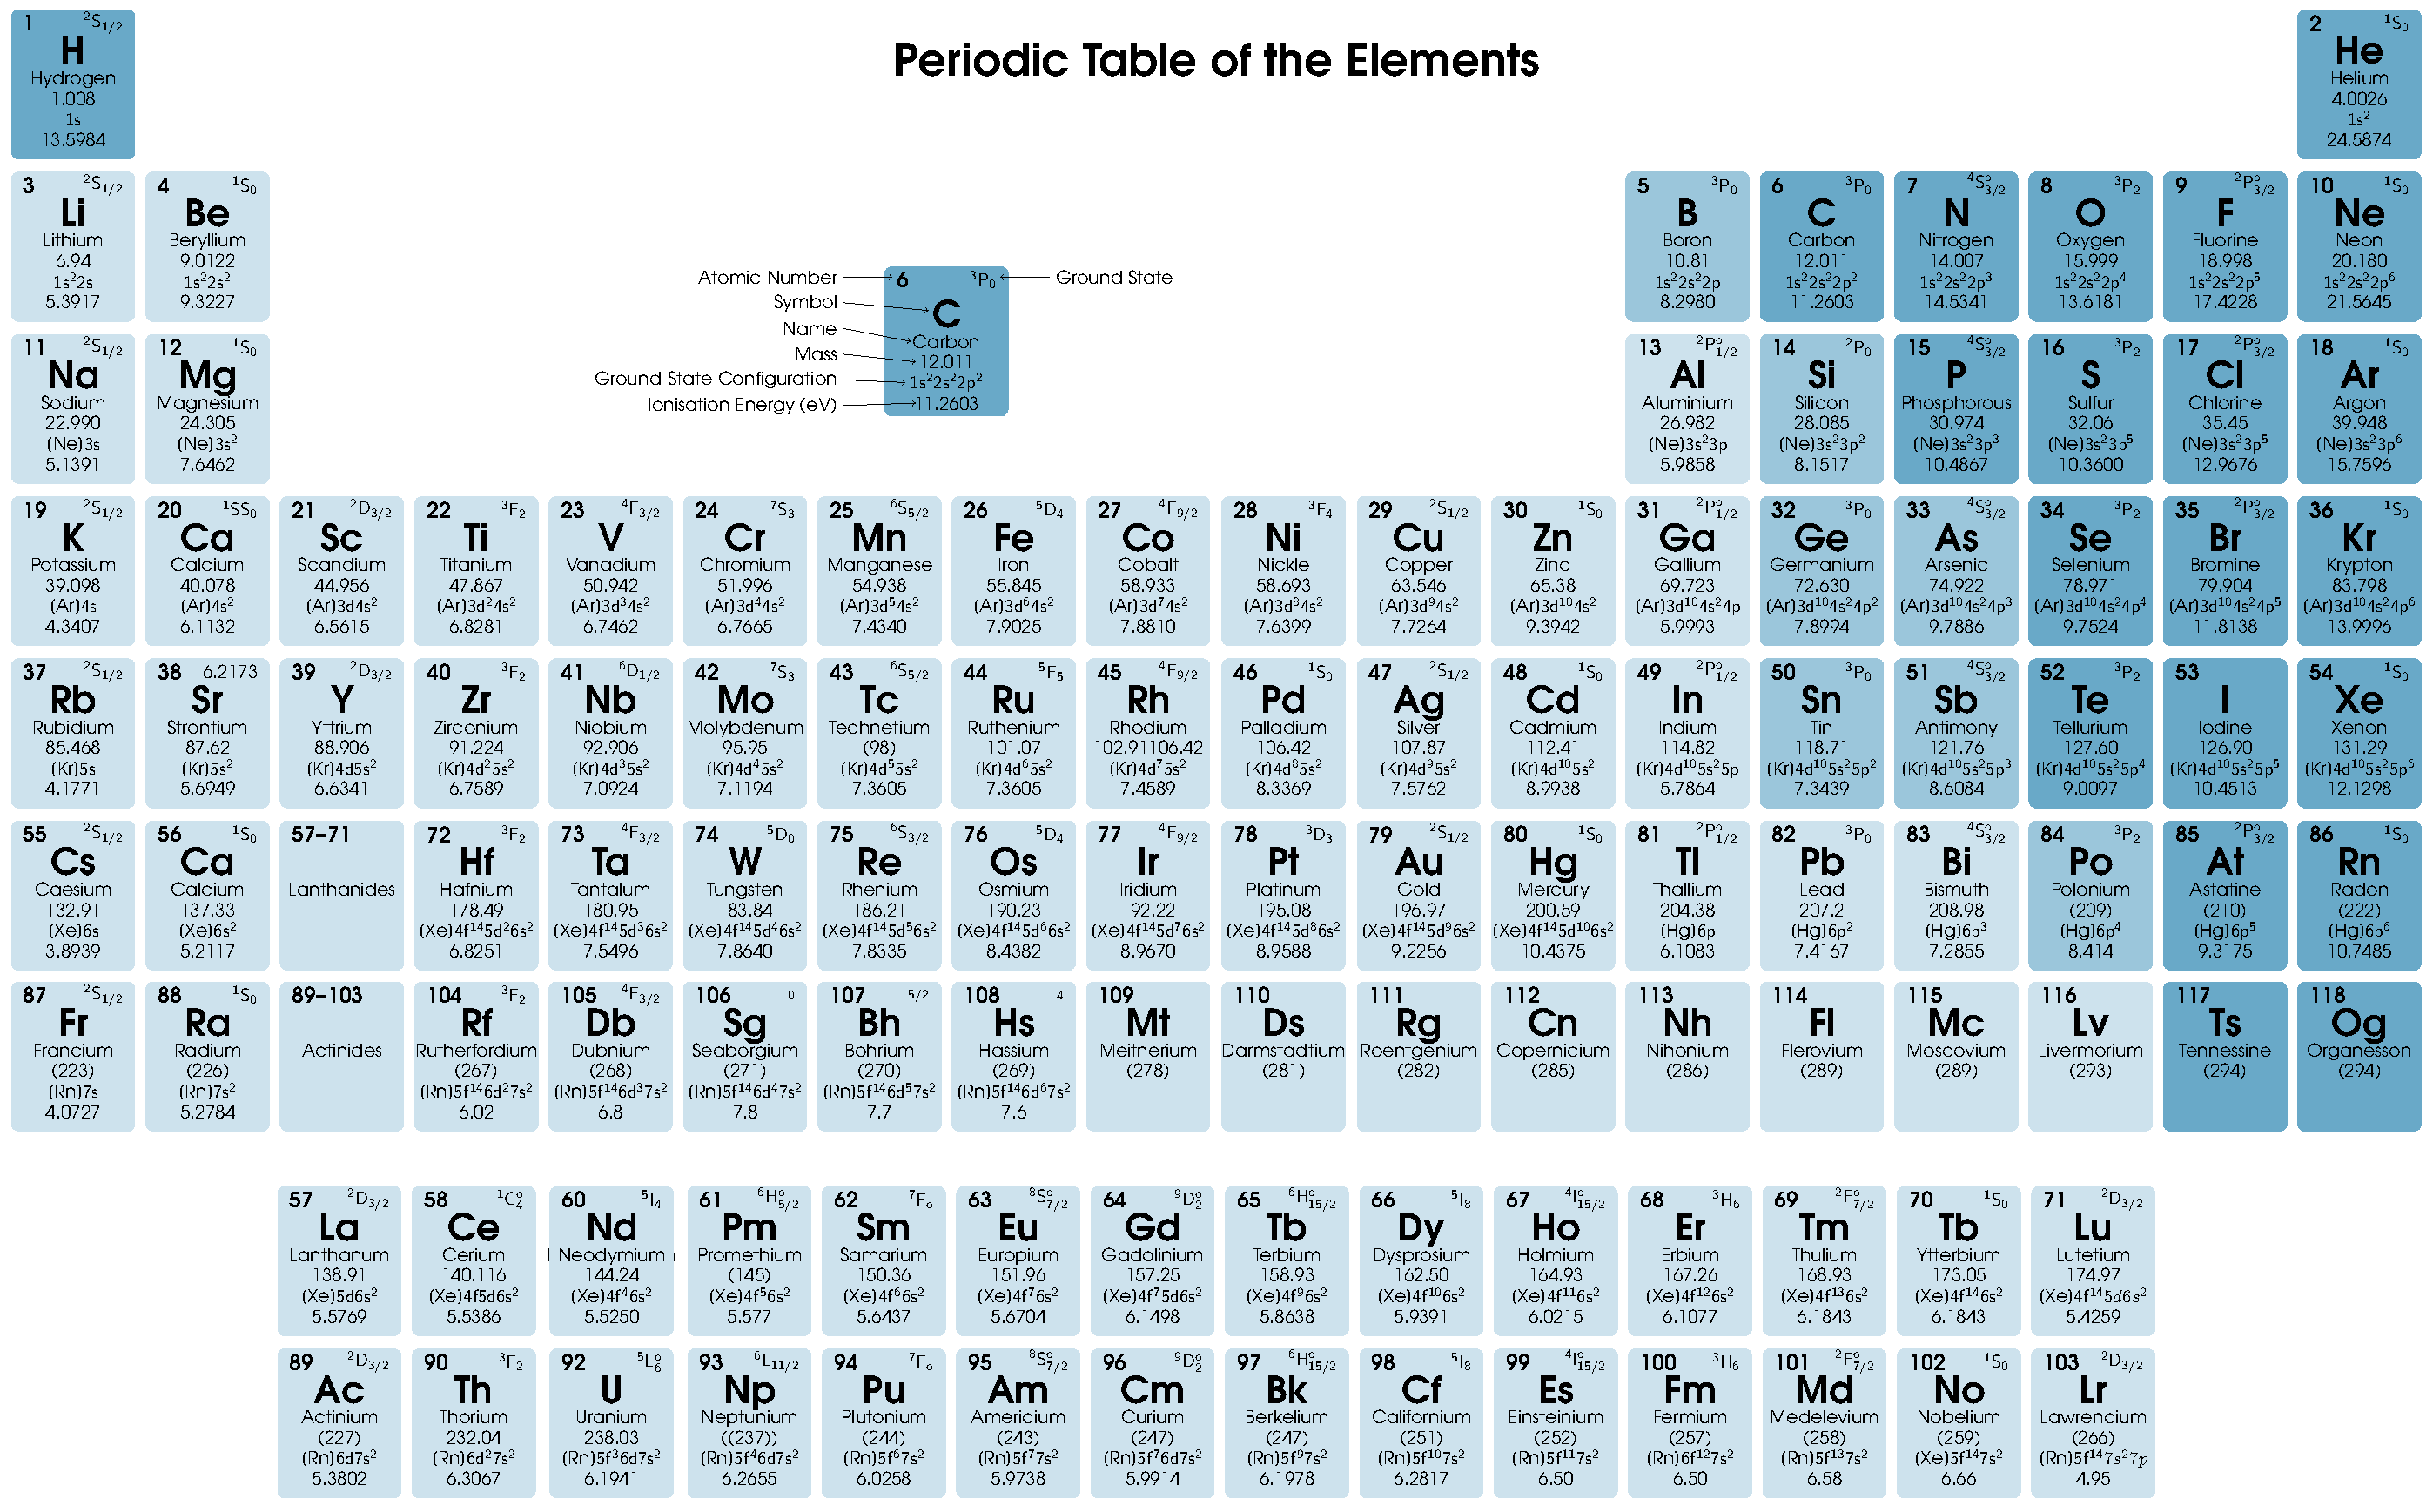
\includegraphics[height=\textwidth, angle=90]{images/periodic-table/periodic-table.pdf}
    \tikzexternaldisable
    \caption[Periodic table.]{Periodic table of the elements: \protect\tikz{\fill[highlight!20] (0, 0) circle [radius = 0.1];} Metals; \protect\tikz{\fill[highlight!40] (0, 0) circle [radius = 0.1];} Metaloids; \protect\tikz{\fill[highlight!60] (0, 0) circle [radius = 0.1];} Nonmetals.}
    \tikzexternalenable
\end{figure}